% !TEX root =big-fish.tex
\chapter{Collision Avoidance}
\label{chap:avoidance}

The collision avoidance algorithm gets triggered when an imminent collision is predicted. Given all the fishes are swimming within the same sphere surface, avoiding a fish without hurting another is guaranteed if the avoiding fish leaves its trajectory's sphere surface to a smaller one (exceptions are treated under section~\ref{sec:recursive-avoidance}). The margin between both spheres gets calculated only once at load time (see section~\ref{subsec:avoidance-margin}).\\

Note that the trajectory's radius gets reduced when avoiding, but never extended, otherwise the fish will be lost of the camera's sight. However in order to keep the  fishes at the same distance from the camera, making it easier to distinguish their sizes and their velocities differences, changing the trajectory's radius should be temporary; as soon as the collision is avoided and the way back is clear, the avoiding fish should return back to its original trajectory.\\

\section{Avoidance phases}
\label{sec:av-phases}

The deviation from the initial trajectory should be smooth by keeping the movement  look continuous and natural. To that end, curvilinear paths towards the target trajectory have been designed as shown in figure~\ref{fig:link}:

\begin{figure}[H]
   \centering
   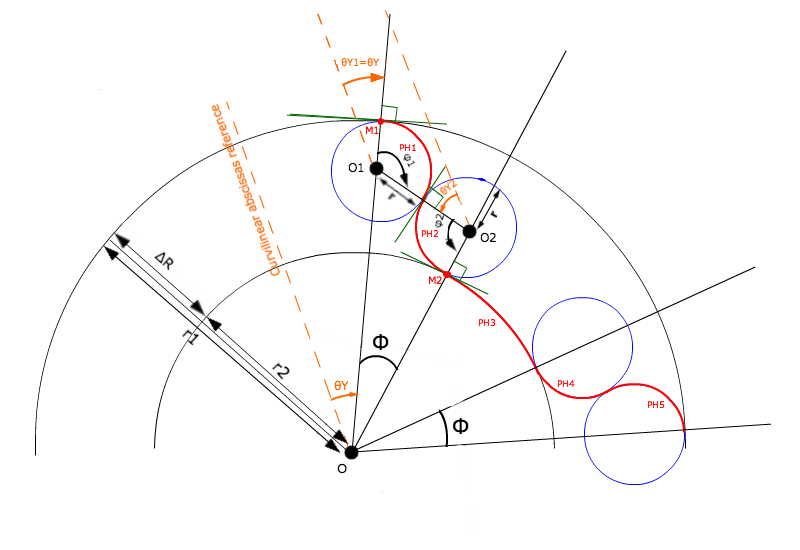
\includegraphics[scale=0.55]{figures/link-trajectory.png}
   \caption{Avoidance link trajectories}
   \label{fig:link}
\end{figure}

The followed path starting from the moment an avoiding fish deviates from its initial trajectory until it returns back, is highlighted in red. It consists of five continuous adjacent arcs, each denoting a separate phase in the avoiding state.

\subsubsection{Phase 1 and Phase 2}

Phase 1 and phase 2 denote the curvilinear link path followed by an avoiding fish towards the target avoidance trajectory. As shown in figure~\ref{fig:link}, the link path is designed as a combination of a couple adjacent circles' arcs, with the goal of making the transition look smooth and natural. Both circles have the same radius r and are respectively adjacent to the start and target trajectories. Both arcs are calculated given the following input:
\begin{itemize}
\item r$_1$ and $r_2$ denoting the respective radiuses for the start and target trajectories. Note that $r_2 = r_1 - \Delta R$, where $\Delta R$ is the safe margin that has been calculated and cached at load time (see section~\ref{subsec:avoidance-margin}).
\item $\theta_Y$ denoting the curvilinear abscissa of the avoiding fish within its swimming trajectory just before it deviates to avoid (see figure~\ref{fig:link}).
\item $M_1$ denoting the position of the avoiding fish just before it deviates to avoid (see figure~\ref{fig:link}).
\item $\Phi = (\overrightarrow{OM_1}, \overrightarrow{OM_2})$ where $M_2$ is the contact point between phase 2 and 3 arcs (see figure~\ref{fig:link}). $\Phi$ is a configurable constant parameter.
\end{itemize}

\bigskip
\bigskip
The results return a couple arcs defined by the following parameters:
\begin{itemize}
\item A radius r (see figure~\ref{fig:link}). r is a solution of the second degree polynomial equation $a r^2 + 2b r + c = 0$ where:
\begin{flalign*}
&\left\{
\begin{array}{lll}
	a = 2 \; (1 - cos\Phi)\\
	b = (1 + cos\Phi) \; (r_1 - r_2)\\
	c = 2 \;r_1 \;r_2 \; cos\Phi - r_1^2 - r_2^2\\
\end{array}
\right.
\;\;\;\;\;\;\Rightarrow r = \frac{-b + \sqrt{b^2 - a \; c}}{a}&
\end{flalign*}

\item $O_i$ the center of the circle carrying the arc (see figure~\ref{fig:link}). Given O is the center of the scene, $O_1$ coordinates can be inferred from the following formula:
\begin{flalign*}
\overrightarrow{OO_1}  = \frac{OM_1 - r}{OM_1} \;.\;\overrightarrow{OM_1}
\end{flalign*}
Inspired by the same logic $O_2$ coordinates can be inferred from the following formula:
\begin{flalign*}
\overrightarrow{OO_2} = \frac{OM_2 + r}{OM_2} \;.\;\overrightarrow{OM_2}
\end{flalign*}
with :
\begin{flalign*}
M_2 = \left(
\begin{array}{ccc}
	r \;.\; sin(\theta_Y + \Phi)\\
	0\\
	r \;.\; cos(\theta_Y + \Phi)\\
\end{array}
\right)_{(\overrightarrow{X}, \overrightarrow{Y}, \overrightarrow{Z})} \; . \; CM
\end{flalign*}
where $(\overrightarrow{X}, \overrightarrow{Y}, \overrightarrow{Z})$ denote the avoiding fish relative rotated axises, and $CM$ being the conversion matrix calculated in section ~\ref{subsec:swimmingstate}.

\item A subtending angle $\varphi_i$ (see figure~\ref{fig:link}). $\varphi_1$ and $\varphi_2$ formulas are the following:
\begin{flalign*}
&\varphi_1 = arccos\left(\frac{\overrightarrow{O_1M_1} \;.\; \overrightarrow{O_1O_2}}{O_1M_1 \;.\; O_1O_2} \right) \;\;\;;\;\;\;
\varphi_2 = arccos\left(\frac{\overrightarrow{O_2O_1} \;.\; \overrightarrow{O_2M_2}}{O_2O_1 \;.\; O_2M_2} \right)&
\end{flalign*}

\item An offset curvilinear abscissa $\theta_{Yi}$ (see figure~\ref{fig:link}). $\theta_{Y1}$ and $\theta_{Y2}$ formulas are the following:
\begin{flalign*}
&\theta_{Y1} = \theta_Y \;\;\;;\;\;\;\; 
\theta_{Y2} = \theta_Y + \Phi - \pi - \varphi_2& 
\end{flalign*}
\end{itemize}

\bigskip
The formulas for phase 4 and 5 arcs will be omitted as they can be easily inspired from the logic above.\\

Note that when following any of the transition paths (i.e. any of phase 1, 2, 4 or 5 arcs), an avoiding fish velocity increases so it avoids the collision fast, which breaks the velocity/response time proportion rule; this should not be a big of an issue as the duration of the transition phases is very short.

\subsubsection{Phase 3}
Phase 3 starts when the avoiding fish arrives to the target avoidance trajectory keeping it safe from collisions.\\

Given phase 3 arc has a smaller radius $r_2$ than $r_1$, the angular velocity $\delta_Y$ should be increased accordingly to maintain the same speed; this can be easily explained by the fact that a turn around a circle having a small radius is executed faster than a turn around a larger circle if the same velocity is maintained; the formula to adapt $\theta_Y$ with the avoidance trajectory is the following: 
\[
\delta_{Y2} \; = \; \frac{r_1}{r_2} \; \delta_{Y1}
\]
where $\delta_{Y1}$ and $\delta_{Y2}$ denote respectively the old and new angular velocities.\\

An avoiding fish in phase 3 keeps an eye on its initial trajectory so that as soon as the way back is clear, it safely returns back thus triggering phase 4 followed by phase 5.

\subsubsection{Phase 4 and phase 5}

Through phase 4 and 5, an avoiding fish returns back to its initial trajectory following the same logic adopted in phase 1 and 2.

\section{Recursive avoidance}
\label{sec:recursive-avoidance}

The scenario illustrated by figure~\ref{fig:link} is the most common; However it has exceptions. In the case where 2 avoiding fishes are waiting for their way back to be cleared and an imminent collision  between both gets predicted the faster fish will avoid again by going through phase 1 followed by phase 2 towards an even smaller radius trajectory. This logic keeps getting applied recursively whenever necessary, until the avoiding fish eventually reaches a trajectory with a minimum radius, smaller than which the fish would collide with the objects in the center of the scene. If this happens, the involved fishes will no longer predict collisions and will just keep checking for their way back to get cleared. This is the only scenario where collisions may occur, but it is very rare, and there must be a busy traffic in the scene (over 20 fishes) so that it happens.\\

The following diagram describes with more details how an avoiding fish switches between phases:\\

\begin{figure}[H]
   \centering
   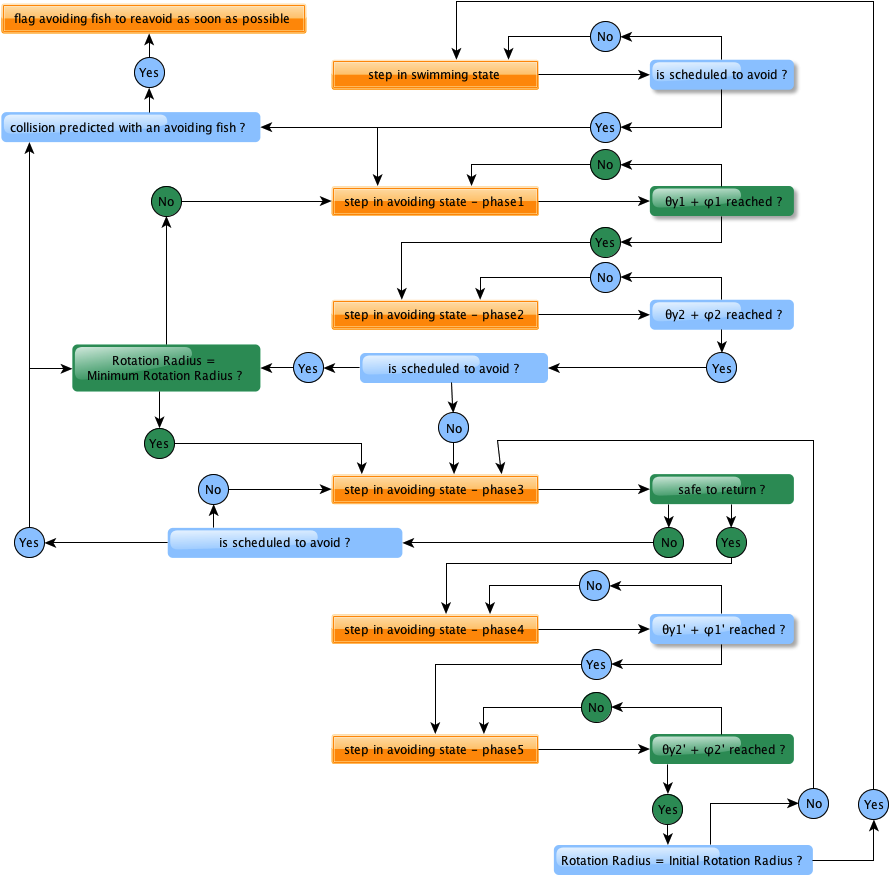
\includegraphics[scale=0.50]{figures/recursive-avoidance.png}
   \caption{Avoidance phases diagram}
   \label{fig:phases}
\end{figure}.\\

The color code used in the diagram is the following:
\begin{itemize}
\item Orange represents actions.
\item Cyan and green represent boolean propositions linked to their eventual values. There is no semantic difference between cyan and green; the simple reason behind using two different colors is to highlight the relationship between propositions and their values given the diagram is relatively dense, thus making it easier to read.
\end{itemize}

The rest of this section will explain some terms used in the diagram; self expressive terms will be omitted.

\subsubsection{Is scheduled to avoid?}
In the beginning of this chapter, it was briefly stated that the collision prediction algorithm filters the collision candidates and forwards them to the avoidance algorithm without much details. In fact whenever a collision is predicted the involved fishes get pushed to a stack of collision candidates. At the end of the frame the stack gets processed to schedule the faster of each couple conflicting fishes to the avoidance state in the next frame. The slower fish will keep its state.

\subsubsection{Flag avoiding fish to reavoid as soon as possible}
Whenever a fish predicts a collision and gets scheduled to avoid in the next frame, just before it switches to phase 1, it estimates whether its path to the avoidance trajectory would result in a collision with any other already avoiding fish, if so the latter gets flagged to re-avoid as soon as possible. If the conflicting fish is on phase 1 or 2, it will re-avoid again as soon as it reaches the target trajectory, otherwise (conflicting fish on phase 3) it will re-avoid immediately in the next frame.

\subsubsection{$\theta_{yi} + \varphi_i$ reached?}
As explained in section~\ref{sec:av-phases}, the link between the initial and target trajectories is made of two adjacent arcs, each having a start angle ($\theta_{yi}$), and a deviation angle ($\varphi_i$) defining the arc's boundaries, which means reaching ($\theta_{yi} + \varphi_i$) ends the corresponding arc thereby triggering a switch of phase.

\subsubsection{Safe to return?}
A fish maintains its state on phase 3 as long as the way back is occupied. Once it gets cleared (safe to return), the fish immediately switches to phase 4 towards its previous trajectory.

\newpage